\chapter{\textit{\acrfull{DTM}}}

\textit{\acrshort{DTM}} прима команде од дебагера помоћу адаптера који те команде преводи у операције протокола који \textit{\acrshort{DTM}} подржава. Имплементирани \textit{\acrshort{DTM}} користи \textit{\acrshort{JTAG}} протокол и примљене команде преводи у приступе \textit{\acrshort{DMI}} магистрали. Принцип функционисања \textit{\acrshort{JTAG}} протокола, као и \textit{\acrshort{DTM}}-а је дат у овом поглављу.

\section{\textit{\acrshort{JTAG}} протокол}

\textit{\acrshort{JTAG}} је комуникациони протокол који \textit{\acrshort{DTM}} користи за комуникацију са адаптером за екстерно дебаговање.
У комуникацији учествују газда (често се назива \textit{\acrfull{ATE}}) и слуга (често се назива \textit{\acrfull{TAP}}), у овом случају адаптер је газда а \textit{\acrshort{DTM}} слуга.
Размена података је серијска и синхрона на сигнал татка који задаје \textit{\acrshort{ATE}}.

Физички, протокол се састоји од 4 линије\footnote{Постоји и верзија са 2 линије али она неће бити обрађивана овде.} а спецификације за екстерно дебаговање понекад додају још опционих линија.

То су:
\begin{itemize}
	\item \textbf{\acrfull{TCK}}, сигнал такта
	\item \textbf{\acrfull{TMS}}, сигнал који управља проласком кроз аутомат стања
	\item \textbf{\acrfull{TDI}}, подаци од \textit{\acrshort{ATE}}-а ка \textit{\acrshort{TAP}}-у
	\item \textbf{\acrfull{TDO}}, подаци од \textit{\acrshort{TAP}}-а ка \textit{\acrshort{ATE}}-у
\end{itemize}
Опционе линије које прописује спецификација:
\begin{itemize}
	\item \textbf{nRESET}, активан у нули, ресетује процесор и периферије
	\item \textbf{n\acrshort{TRST}}, активан у нули, ресетује \textit{\acrshort{TAP}}
\end{itemize}

Концептуално \textit{\acrshort{TAP}} поседује шифт регистар подесиве ширине\footnote{Спецификација користи више шифт регистара али аутор сматра да је репрезентација са једним шифт регистром лакша за разумевање.} и регистар инструкције, проласком кроз аутомат стања (приказан на слици \ref{fig:jtag}) у одређеним тренуцима се врши паралелни упис или читање или серијски упис и читање шифт регистра. Аутомат стања унутар \textit{\acrshort{TAP}}-а мења стање на узлазну ивицу сигнала такта, стање у које прелази је спецификовано вредношћу сигнала \textbf{\acrshort{TMS}} у том тренутку.
Стања од интереса су \textbf{Capture-\acrshort{IR}}, \textbf{Capture-\acrshort{DR}}, \textbf{Shift-\acrshort{IR}}, \textbf{Shift-\acrshort{DR}}, \textbf{Update-\acrshort{IR}} и \textbf{Update-\acrshort{DR}}. 
У стању \textbf{Capture-\acrshort{IR}} се на узлазну ивицу \textbf{\acrshort{TCK}} у шифт регистар паралелно учитава произвољан низ битова ширине инструкцијског регистра (параметар \textit{\acrshort{TAP}}-а, мора бити константан) чија два најнижа бита морају бити 01 и ширина шифт регистра се поставља на ширину инструкцијског регистра. У стању \textbf{Capture-\acrshort{DR}} се на узлазну ивицу \textbf{\acrshort{TCK}} у шифт регистар паралелно учитава вредност регистра за податке спецификована тренутном вредношћу инструкцијског регистра и ширина шифт регистра се поставља на ширину тог регистра (мора бити фиксна у зависности од инструкције, различите инструкције могу имати регистре различите дужине). У стањима \textbf{Shift-\acrshort{IR}} и \textbf{Shift-\acrshort{DR}} се на узлазну ивицу \textbf{\acrshort{TCK}} у шифт регистар серијски уписује на место највишег бита вредност \textbf{\acrshort{TDI}}, док се на силазну ивицу \textbf{\acrshort{TCK}} на линију \textbf{\acrshort{TDO}} поставља вредност најнижег бита шифт регистра. У стањима \textbf{Update-\acrshort{IR}} и \textbf{Update-\acrshort{DR}} се на силазну ивицу \textbf{\acrshort{TCK}} паралелно уписује у инструкцијски регистар или регистар података спецификован тренутном вредношћу инструкцијског регистра. При упису регистар за податке, \textit{\acrshort{TAP}} може такође извршити произвољну акцију (као што је операција на магистрали).

\begin{figure}[h!]
	\centering
	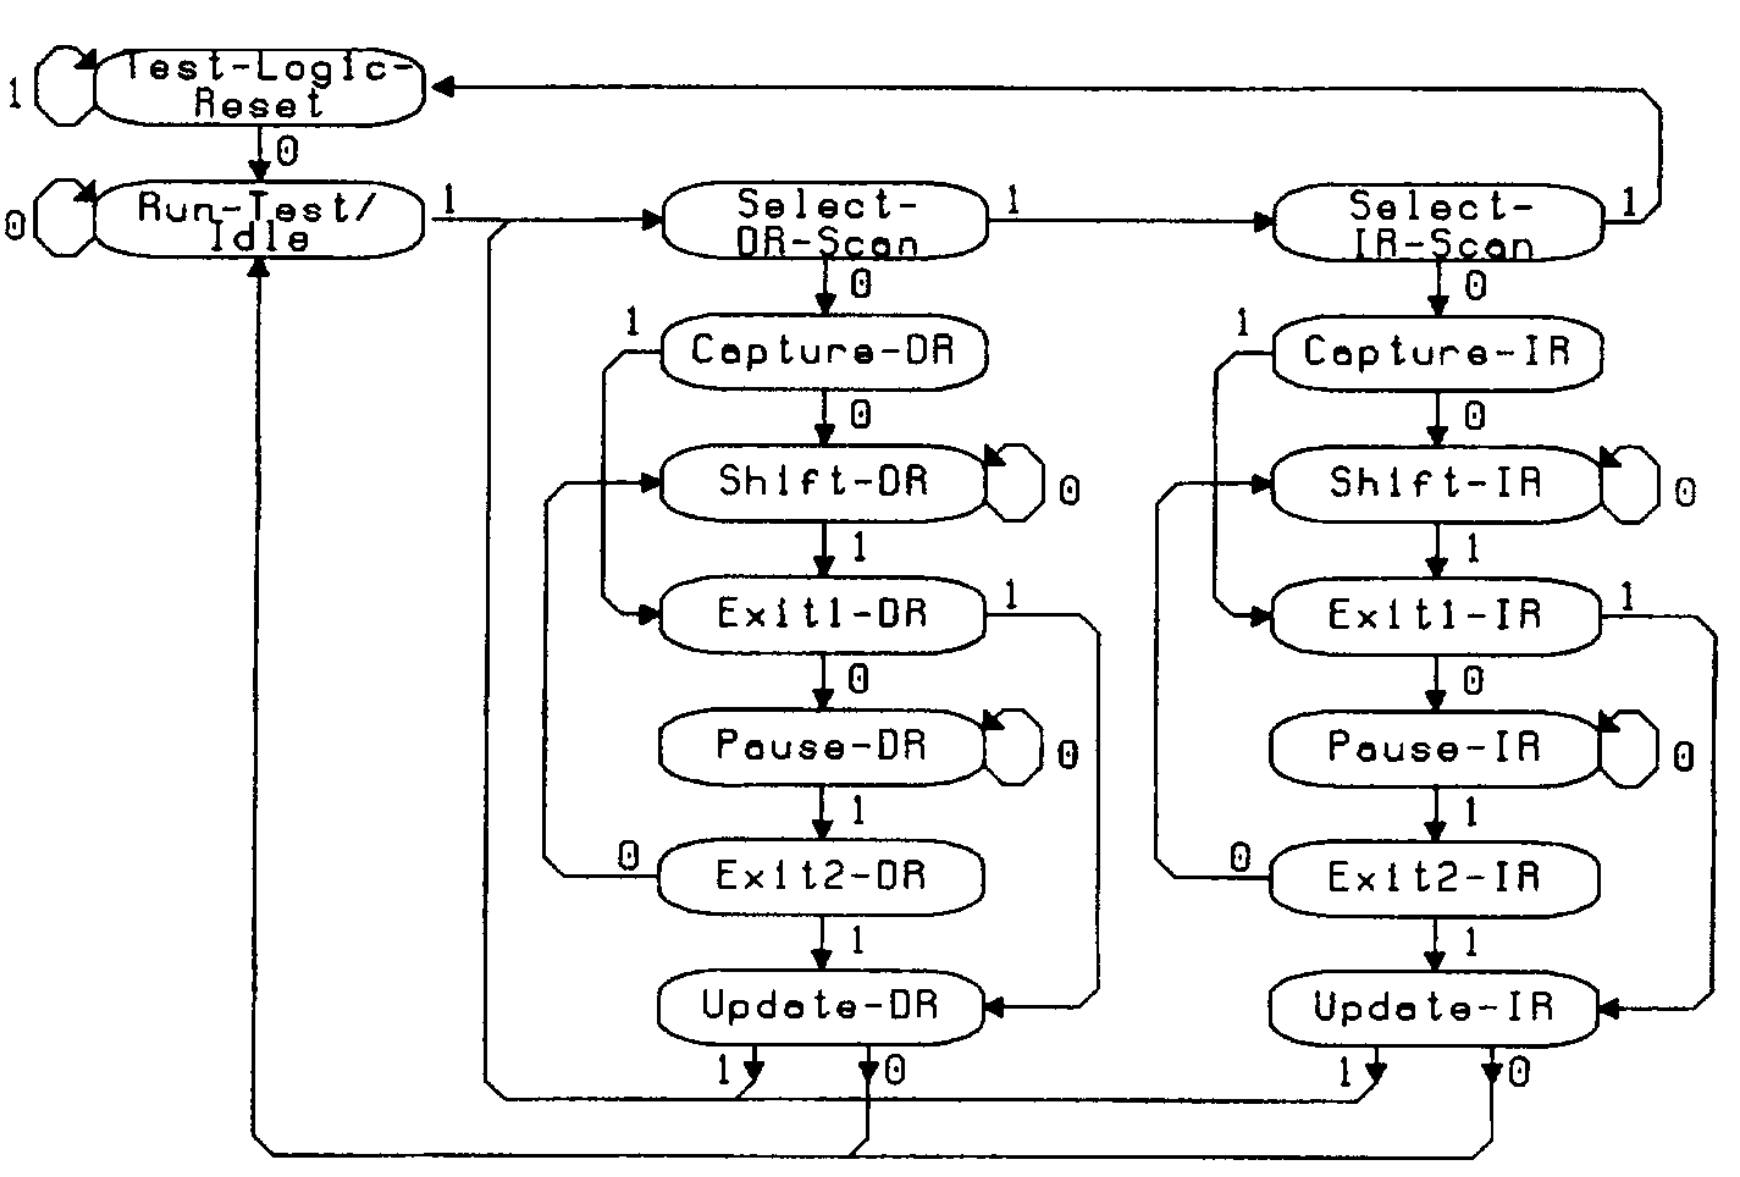
\includegraphics[width=0.7\textwidth]{jtag}
	\caption{Аутомат стања \textit{\acrshort{JTAG}} протокола \cite{jtag_spec}}
	\label{fig:jtag}
\end{figure}

У \textit{\acrshort{JTAG}} протоколу се комбинација инструкцијског регистра и регистара за податке може замислити као меморија где вредност инструкцијског регистра представља адресу а регистри за податке представљају податке, разлика је што различити регистри за податке могу бити различите ширине.

\рисцв{} спецификација \cite{debug_spec} захтева да компатибилни \textit{\acrshort{TAP}} имплементира \textbf{BYPASS} и \textbf{IDCODE} \textit{\acrshort{JTAG}} инструкције, као и \textbf{\acrshort{DTMCS}} и \textbf{\acrshort{DMI}} које су специфичне за \рисцв{} \textit{\acrshort{DTM}}. \textbf{BYPASS} инструкција представља регистар намењен само за читање ширине једног бита чија је вредност 0. Намена ове инструкције је скраћивање ланца шифт регистара уколико је више \textit{\acrshort{TAP}}-ова редно повезано и \textit{\acrshort{ATE}} задаје команду неком другом уређају. Инструкција \textbf{IDCODE} представља регистар намењен само за читање ширине 32 бита и садржи јединствени идентификатор \textit{\acrshort{TAP}}-а. \textbf{DTMCS} омогућава приступ статусу \textit{\acrshort{DTM}}-а (бити статуса су намењени само за читање) и пружа два бита за ресетовање \textit{\acrshort{DTM}}-а. Један бит прекида тренутну \textit{\acrshort{DMI}} трансакцију а други ресетује индикатор грешке. Како су у овој имплементацији \textit{\acrshort{DMI}} трансакције трајања једног такта, \textit{\acrshort{ATE}} не може стићи да приступи неком регистру \textit{\acrshort{DTM}}-а док је трансакција у току, те је немогуће прекинути трансакцију у току или изазвати грешку па бити за ресет нису имплементирани. Регистар \textbf{\acrshort{DMI}} инструкције је ширине 34 бита + ширина адресе \textit{\acrshort{DMI}} адресног простора. Уписом у овај регистар \textit{\acrshort{ATE}} може (у зависности од поља операције) извршити приступ преко \textit{\acrshort{DMI}} магистрале. При следећем читању \textbf{\acrshort{DMI}} регистра, у њему се налази информација о успешности приступа и прочитана вредност уколико је била реч о операцији читања.

\section{Имплементација \textit{\acrshort{DTM}}-a}

Како су улазни сигнали асинхрони у односу на унутрашњи сигнал такта, они прво пролазе кроз ланац за синхронизацију где се за сигнале \textbf{\acrfull{TMS}}, \textbf{\acrfull{TDI}} и \textbf{\acrfull{TDO}} користи вредност другог регистра у ланцу а за сигнал \textbf{\acrfull{TCK}} се детектују узлазне и силазне ивице коришћењем вредности другог и трећег регистра у ланцу. Имплементација саме \textit{\acrshort{TAP}} логике се своди на имплементацију аутомата стања, шифт регистра и учитавања правилних вредности у шифт регистар, инструкцијски регистар и регистре за податке, као што је објашњено изнад.

Само извршавање операција на \textit{\acrshort{DMI}} магистрали се своди на постављање одговарајућих делова \textbf{\acrshort{DMI}} регистра на линије магистрале, такт након уписа у \textbf{\acrshort{DMI}} регистар и учитавања информације о успешности приступа и прочитане вредности (уколико се радило о операцији читања) у \textbf{\acrshort{DMI}} регистар такт касније.